\documentclass[border=5pt]{standalone}
\usepackage{tikz}
\usepackage{amsmath}
\usetikzlibrary{calc, positioning, arrows.meta}
\begin{document}
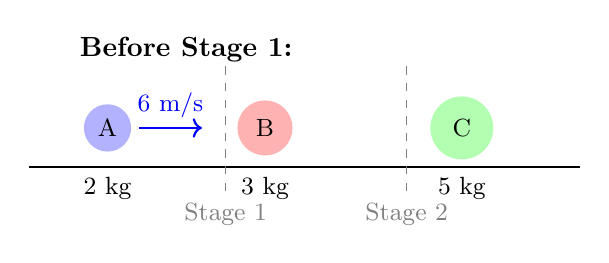
\begin{tikzpicture}[scale=1.0]
  % Initial configuration
  \node at (-1,1.5) {\textbf{Before Stage 1:}};

  % Sphere A moving
  \fill[blue!30] (-2,0.5) circle (0.3);
  \node at (-2,0.5) {\small A};
  \draw[->, thick, blue] (-1.6,0.5) -- (-0.8,0.5) node[midway, above] {\small $6$ m/s};

  % Sphere B at rest
  \fill[red!30] (0,0.5) circle (0.35);
  \node at (0,0.5) {\small B};

  % Sphere C at rest
  \fill[green!30] (2.5,0.5) circle (0.4);
  \node at (2.5,0.5) {\small C};

  % Ground line
  \draw[thick] (-3,0) -- (4,0);

  % Labels
  \node[below] at (-2,0) {\small $2$ kg};
  \node[below] at (0,0) {\small $3$ kg};
  \node[below] at (2.5,0) {\small $5$ kg};

  % Stage indicators
  \draw[dashed, gray] (-0.5,-0.3) -- (-0.5,1.3);
  \node[gray] at (-0.5,-0.6) {\small Stage 1};

  \draw[dashed, gray] (1.8,-0.3) -- (1.8,1.3);
  \node[gray] at (1.8,-0.6) {\small Stage 2};
\end{tikzpicture}
\end{document}
